\documentclass{../../ktane-mod}


\begin{document}

\begin{module}{
  moduleName=Mazes,
  indexString=Mazes,
  imageResource=mazes_img.pdf,
  interactions=\keysymbol
}
{
  This seems to be some kind of maze, probably stolen off a restaurant placemat.
}

\begin{bulletlist}
  \bulletitem{Have the defuser name any of the circular markings using a letter for columns and a number for lines.}
  \bulletitem{Find the matching maze using the helpful chart on the left below. The black square identifies which of the nine mazes matches the given circle coordinate.}
  \bulletitem{The defuser must navigate the white light to the red triangle using the arrow buttons.}
  \bulletitem{\textbf{WARNING:} Do not cross the lines of the maze. These lines are invisible on the bomb.}
\end{bulletlist}

\vspace{0.2cm}

% Two-section horizontal layout  
\begin{minipage}[t]{0.13\textwidth}
  \phantom{x}% Establish baseline for [t] alignment
  % Left section: 2-column table without gridlines
  \newcommand{\gridscale}{0.65}
  \begin{NiceTabular}{m{.45cm}m{.85cm}}
    A1 & \begin{tikzpicture}[scale=\gridscale, baseline=-0.2cm]
      \draw[step=0.33cm,black,thin] (0,0) grid (1,1);
      \fill[black] (0,0.33) rectangle (0.33,0.67); % l (left)
    \end{tikzpicture} \\
    A2 & \begin{tikzpicture}[scale=\gridscale, baseline=-0.2cm]
      \draw[step=0.33cm,black,thin] (0,0) grid (1,1);
      \fill[black] (0,0.67) rectangle (0.33,1); % tl (top-left)
    \end{tikzpicture} \\
    A4 & \begin{tikzpicture}[scale=\gridscale, baseline=-0.2cm]
      \draw[step=0.33cm,black,thin] (0,0) grid (1,1);
      \fill[black] (0,0.33) rectangle (0.33,0.67); % l (left)
    \end{tikzpicture} \\
    A5 & \begin{tikzpicture}[scale=\gridscale, baseline=-0.2cm]
      \draw[step=0.33cm,black,thin] (0,0) grid (1,1);
      \fill[black] (0.67,0) rectangle (1,0.33); % br (bottom-right)
    \end{tikzpicture} \\
    B1 & \begin{tikzpicture}[scale=\gridscale, baseline=-0.2cm]
      \draw[step=0.33cm,black,thin] (0,0) grid (1,1);
      \fill[black] (0,0) rectangle (0.33,0.33); % bl (bottom-left)
    \end{tikzpicture} \\
    B4 & \begin{tikzpicture}[scale=\gridscale, baseline=-0.2cm]
      \draw[step=0.33cm,black,thin] (0,0) grid (1,1);
      \fill[black] (0.33,0.67) rectangle (0.67,1); % t (top)
    \end{tikzpicture} \\
    B6 & \begin{tikzpicture}[scale=\gridscale, baseline=-0.2cm]
      \draw[step=0.33cm,black,thin] (0,0) grid (1,1);
      \fill[black] (0,0) rectangle (0.33,0.33); % bl (bottom-left)
    \end{tikzpicture} \\
    C2 & \begin{tikzpicture}[scale=\gridscale, baseline=-0.2cm]
      \draw[step=0.33cm,black,thin] (0,0) grid (1,1);
      \fill[black] (0.67,0) rectangle (1,0.33); % br (bottom-right)
    \end{tikzpicture} \\
    C4 & \begin{tikzpicture}[scale=\gridscale, baseline=-0.2cm]
      \draw[step=0.33cm,black,thin] (0,0) grid (1,1);
      \fill[black] (0.33,0) rectangle (0.67,0.33); % b (bottom)
    \end{tikzpicture} \\
    C5 & \begin{tikzpicture}[scale=\gridscale, baseline=-0.2cm]
      \draw[step=0.33cm,black,thin] (0,0) grid (1,1);
      \fill[black] (0.67,0.33) rectangle (1,0.67); % r (right)
    \end{tikzpicture} \\
    D1 & \begin{tikzpicture}[scale=\gridscale, baseline=-0.2cm]
      \draw[step=0.33cm,black,thin] (0,0) grid (1,1);
      \fill[black] (0.33,0) rectangle (0.67,0.33); % b (bottom)
    \end{tikzpicture} \\
    D4 & \begin{tikzpicture}[scale=\gridscale, baseline=-0.2cm]
      \draw[step=0.33cm,black,thin] (0,0) grid (1,1);
      \fill[black] (0.67,0.67) rectangle (1,1); % tr (top-right)
    \end{tikzpicture} \\
    D6 & \begin{tikzpicture}[scale=\gridscale, baseline=-0.2cm]
      \draw[step=0.33cm,black,thin] (0,0) grid (1,1);
      \fill[black] (0.33,0.33) rectangle (0.67,0.67); % c (center)
    \end{tikzpicture} \\
    E1 & \begin{tikzpicture}[scale=\gridscale, baseline=-0.2cm]
      \draw[step=0.33cm,black,thin] (0,0) grid (1,1);
      \fill[black] (0.67,0.33) rectangle (1,0.67); % r (right)
    \end{tikzpicture} \\
    E2 & \begin{tikzpicture}[scale=\gridscale, baseline=-0.2cm]
      \draw[step=0.33cm,black,thin] (0,0) grid (1,1);
      \fill[black] (0.33,0.67) rectangle (0.67,1); % t (top)
    \end{tikzpicture} \\
    E3 & \begin{tikzpicture}[scale=\gridscale, baseline=-0.2cm]
      \draw[step=0.33cm,black,thin] (0,0) grid (1,1);
      \fill[black] (0.33,0.33) rectangle (0.67,0.67); % c (center)
    \end{tikzpicture} \\
    F3 & \begin{tikzpicture}[scale=\gridscale, baseline=-0.2cm]
      \draw[step=0.33cm,black,thin] (0,0) grid (1,1);
      \fill[black] (0,0.67) rectangle (0.33,1); % tl (top-left)
    \end{tikzpicture} \\
    F4 & \begin{tikzpicture}[scale=\gridscale, baseline=-0.2cm]
      \draw[step=0.33cm,black,thin] (0,0) grid (1,1);
      \fill[black] (0.67,0.67) rectangle (1,1); % tr (top-right)
    \end{tikzpicture} \\
  \end{NiceTabular}
\end{minipage}%
\hfill%
\begin{minipage}[t]{0.82\textwidth}
  \phantom{x}% Establish baseline for [t] alignment
  % Right section: 9 mazes using simple approach
  \centering
  
  % Define maze cell with gray dot
  \newcommand{\mazecell}{\begin{tikzpicture}[scale=0.15, baseline=0cm]
    \fill[gray] (0.5,0.5) circle (0.08);
  \end{tikzpicture}}
  
  % Create 9 mazes in a 3x3 grid using tikz
  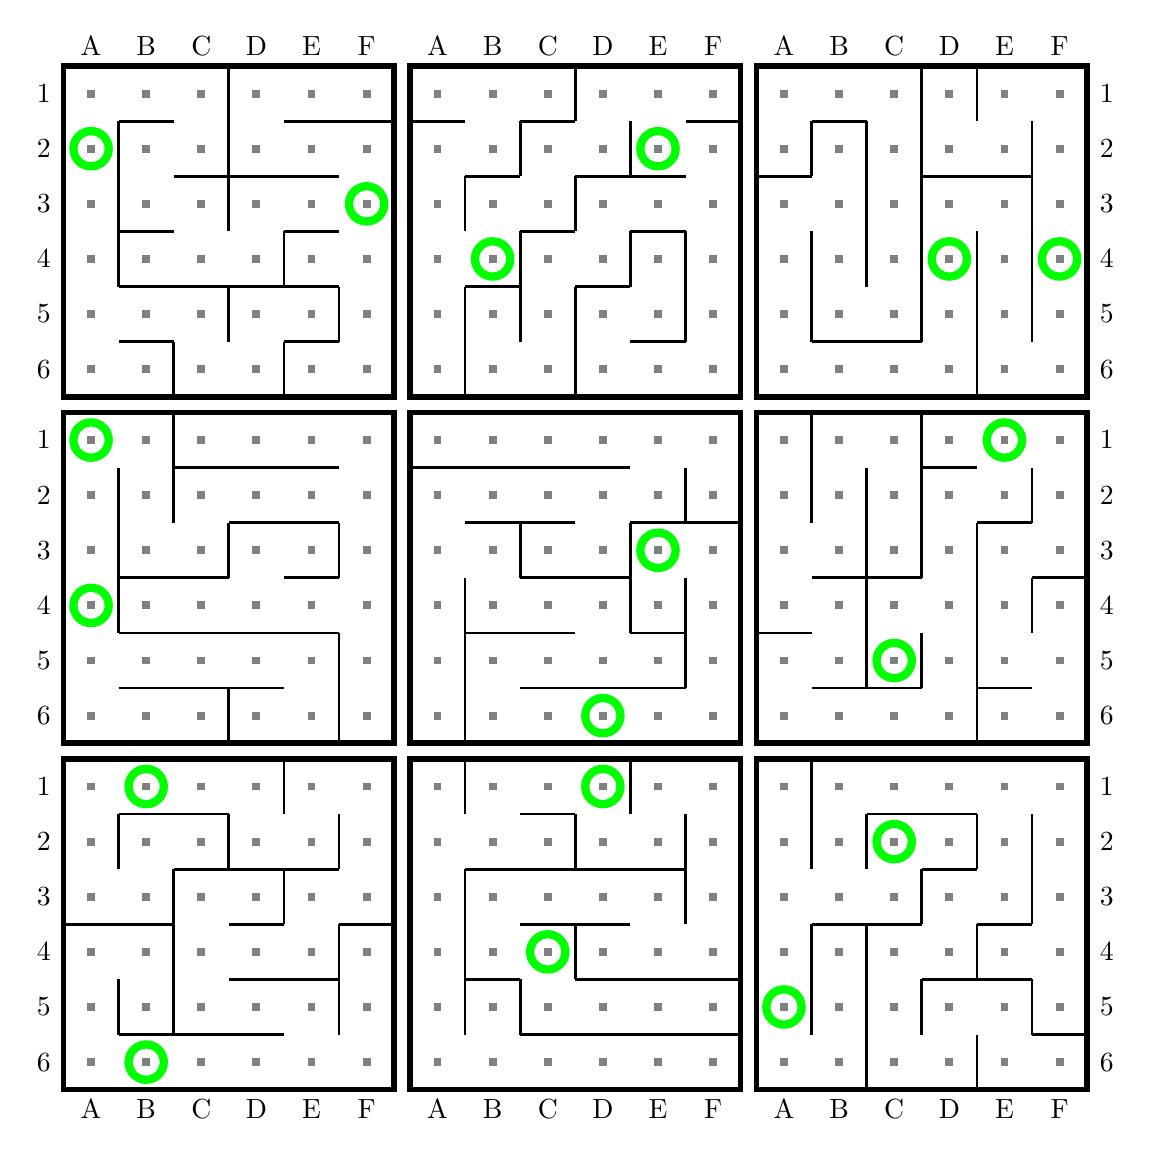
\begin{tikzpicture}
    % Define maze size and spacing (each cell = 7mm, 6x6 = 42mm = 4.2cm)
    \def\mazesize{4.2}
    \def\spacing{4.4}
    
    % Draw all 9 maze outlines and contents
    \foreach \row in {0,1,2} {
      \foreach \col in {0,1,2} {
        % Calculate position
        \pgfmathsetmacro{\xpos}{\col * \spacing}
        \pgfmathsetmacro{\ypos}{-\row * \spacing}
        
        % Draw maze outline
        \draw[line width=2pt] (\xpos,\ypos) rectangle (\xpos+\mazesize,\ypos+\mazesize);
        
        % Add column labels (top for all mazes, bottom for all mazes)
        \ifnum\row=0
          \foreach \c [count=\ci] in {A,B,C,D,E,F} {
            \pgfmathsetmacro{\colx}{\xpos + (\ci-1)*\mazesize/6 + \mazesize/12}
            \node at (\colx, \ypos+\mazesize+0.25) {\c};
          }
        \fi
        \ifnum\row=2
          \foreach \c [count=\ci] in {A,B,C,D,E,F} {
            \pgfmathsetmacro{\colx}{\xpos + (\ci-1)*\mazesize/6 + \mazesize/12}
            \node at (\colx, \ypos-0.25) {\c};
          }
        \fi
        
        % Add row labels (left for all mazes, right for all mazes)
        \ifnum\col=0
          \foreach \r [count=\ri] in {1,2,3,4,5,6} {
            \pgfmathsetmacro{\rowy}{\ypos + \mazesize - (\ri-1)*\mazesize/6 - \mazesize/12}
            \node at (\xpos-0.25, \rowy) {\r};
          }
        \fi
        \ifnum\col=2
          \foreach \r [count=\ri] in {1,2,3,4,5,6} {
            \pgfmathsetmacro{\rowy}{\ypos + \mazesize - (\ri-1)*\mazesize/6 - \mazesize/12}
            \node at (\xpos+\mazesize+0.25, \rowy) {\r};
          }
        \fi
        
        % Fill maze with gray squares
        \foreach \x in {0,1,2,3,4,5} {
          \foreach \y in {0,1,2,3,4,5} {
            \pgfmathsetmacro{\dotx}{\xpos + (\x+0.5)*\mazesize/6}
            \pgfmathsetmacro{\doty}{\ypos + (\y+0.5)*\mazesize/6}
            \fill[gray] (\dotx-0.05,\doty-0.05) rectangle (\dotx+0.05,\doty+0.05);
          }
        }
        
        % Draw maze walls based on patterns
        % Maze 1 (top-left, row=0, col=0): 
        % x b r x b b / r x br b b x / r b r x b x / r b b br b x / x b r x br x / x r x r x x
        \ifnum\row=0\ifnum\col=0
          % Row 0: x b r x b b
          \pgfmathsetmacro{\cellx}{\xpos + 1*\mazesize/6}
          \pgfmathsetmacro{\celly}{\ypos + \mazesize - 1*\mazesize/6}
          \draw[black, line width=1pt] (\cellx,\celly) -- (\cellx+\mazesize/6,\celly); % b
          \pgfmathsetmacro{\cellx}{\xpos + 2*\mazesize/6}
          \draw[black, line width=1pt] (\cellx+\mazesize/6,\celly) -- (\cellx+\mazesize/6,\celly+\mazesize/6); % r
          \pgfmathsetmacro{\cellx}{\xpos + 4*\mazesize/6}
          \draw[black, line width=1pt] (\cellx,\celly) -- (\cellx+\mazesize/6,\celly); % b
          \pgfmathsetmacro{\cellx}{\xpos + 5*\mazesize/6}
          \draw[black, line width=1pt] (\cellx,\celly) -- (\cellx+\mazesize/6,\celly); % b
          
          % Row 1: r x br b b x
          \pgfmathsetmacro{\cellx}{\xpos + 0*\mazesize/6}
          \pgfmathsetmacro{\celly}{\ypos + \mazesize - 2*\mazesize/6}
          \draw[black, line width=1pt] (\cellx+\mazesize/6,\celly) -- (\cellx+\mazesize/6,\celly+\mazesize/6); % r
          \pgfmathsetmacro{\cellx}{\xpos + 2*\mazesize/6}
          \draw[black, line width=1pt] (\cellx,\celly) -- (\cellx+\mazesize/6,\celly); % br-b
          \draw[black, line width=1pt] (\cellx+\mazesize/6,\celly) -- (\cellx+\mazesize/6,\celly+\mazesize/6); % br-r
          \pgfmathsetmacro{\cellx}{\xpos + 3*\mazesize/6}
          \draw[black, line width=1pt] (\cellx,\celly) -- (\cellx+\mazesize/6,\celly); % b
          \pgfmathsetmacro{\cellx}{\xpos + 4*\mazesize/6}
          \draw[black, line width=1pt] (\cellx,\celly) -- (\cellx+\mazesize/6,\celly); % b
          
          % Row 2: r b r x b x
          \pgfmathsetmacro{\cellx}{\xpos + 0*\mazesize/6}
          \pgfmathsetmacro{\celly}{\ypos + \mazesize - 3*\mazesize/6}
          \draw[black, line width=1pt] (\cellx+\mazesize/6,\celly) -- (\cellx+\mazesize/6,\celly+\mazesize/6); % r
          \pgfmathsetmacro{\cellx}{\xpos + 1*\mazesize/6}
          \draw[black, line width=1pt] (\cellx,\celly) -- (\cellx+\mazesize/6,\celly); % b
          \pgfmathsetmacro{\cellx}{\xpos + 2*\mazesize/6}
          \draw[black, line width=1pt] (\cellx+\mazesize/6,\celly) -- (\cellx+\mazesize/6,\celly+\mazesize/6); % r
          \pgfmathsetmacro{\cellx}{\xpos + 4*\mazesize/6}
          \draw[black, line width=1pt] (\cellx,\celly) -- (\cellx+\mazesize/6,\celly); % b
          
          % Row 3: r b b br b x
          \pgfmathsetmacro{\cellx}{\xpos + 0*\mazesize/6}
          \pgfmathsetmacro{\celly}{\ypos + \mazesize - 4*\mazesize/6}
          \draw[black, line width=1pt] (\cellx+\mazesize/6,\celly) -- (\cellx+\mazesize/6,\celly+\mazesize/6); % r
          \pgfmathsetmacro{\cellx}{\xpos + 1*\mazesize/6}
          \draw[black, line width=1pt] (\cellx,\celly) -- (\cellx+\mazesize/6,\celly); % b
          \pgfmathsetmacro{\cellx}{\xpos + 2*\mazesize/6}
          \draw[black, line width=1pt] (\cellx,\celly) -- (\cellx+\mazesize/6,\celly); % b
          \pgfmathsetmacro{\cellx}{\xpos + 3*\mazesize/6}
          \draw[black, line width=1pt] (\cellx,\celly) -- (\cellx+\mazesize/6,\celly); % br-b
          \draw[black, line width=1pt] (\cellx+\mazesize/6,\celly) -- (\cellx+\mazesize/6,\celly+\mazesize/6); % br-r
          \pgfmathsetmacro{\cellx}{\xpos + 4*\mazesize/6}
          \draw[black, line width=1pt] (\cellx,\celly) -- (\cellx+\mazesize/6,\celly); % b
          
          % Row 4: x b r x br x
          \pgfmathsetmacro{\cellx}{\xpos + 1*\mazesize/6}
          \pgfmathsetmacro{\celly}{\ypos + \mazesize - 5*\mazesize/6}
          \draw[black, line width=1pt] (\cellx,\celly) -- (\cellx+\mazesize/6,\celly); % b
          \pgfmathsetmacro{\cellx}{\xpos + 2*\mazesize/6}
          \draw[black, line width=1pt] (\cellx+\mazesize/6,\celly) -- (\cellx+\mazesize/6,\celly+\mazesize/6); % r
          \pgfmathsetmacro{\cellx}{\xpos + 4*\mazesize/6}
          \draw[black, line width=1pt] (\cellx,\celly) -- (\cellx+\mazesize/6,\celly); % br-b
          \draw[black, line width=1pt] (\cellx+\mazesize/6,\celly) -- (\cellx+\mazesize/6,\celly+\mazesize/6); % br-r
          
          % Row 5: x r x r x x
          \pgfmathsetmacro{\cellx}{\xpos + 1*\mazesize/6}
          \pgfmathsetmacro{\celly}{\ypos + \mazesize - 6*\mazesize/6}
          \draw[black, line width=1pt] (\cellx+\mazesize/6,\celly) -- (\cellx+\mazesize/6,\celly+\mazesize/6); % r
          \pgfmathsetmacro{\cellx}{\xpos + 3*\mazesize/6}
          \draw[black, line width=1pt] (\cellx+\mazesize/6,\celly) -- (\cellx+\mazesize/6,\celly+\mazesize/6); % r
        \fi\fi
        
        % Maze 2 (top-center, row=0, col=1):
        % b x br x x b / x br x br b x / r x br x b x / x br x br r x / r r r x br x / r x r x x x
        \ifnum\row=0\ifnum\col=1
          % Row 0: b x br x x b
          \pgfmathsetmacro{\cellx}{\xpos + 0*\mazesize/6}
          \pgfmathsetmacro{\celly}{\ypos + \mazesize - 1*\mazesize/6}
          \draw[black, line width=1pt] (\cellx,\celly) -- (\cellx+\mazesize/6,\celly); % b
          \pgfmathsetmacro{\cellx}{\xpos + 2*\mazesize/6}
          \draw[black, line width=1pt] (\cellx,\celly) -- (\cellx+\mazesize/6,\celly); % br-b
          \draw[black, line width=1pt] (\cellx+\mazesize/6,\celly) -- (\cellx+\mazesize/6,\celly+\mazesize/6); % br-r
          \pgfmathsetmacro{\cellx}{\xpos + 5*\mazesize/6}
          \draw[black, line width=1pt] (\cellx,\celly) -- (\cellx+\mazesize/6,\celly); % b
          
          % Row 1: x br x br b x
          \pgfmathsetmacro{\cellx}{\xpos + 1*\mazesize/6}
          \pgfmathsetmacro{\celly}{\ypos + \mazesize - 2*\mazesize/6}
          \draw[black, line width=1pt] (\cellx,\celly) -- (\cellx+\mazesize/6,\celly); % br-b
          \draw[black, line width=1pt] (\cellx+\mazesize/6,\celly) -- (\cellx+\mazesize/6,\celly+\mazesize/6); % br-r
          \pgfmathsetmacro{\cellx}{\xpos + 3*\mazesize/6}
          \draw[black, line width=1pt] (\cellx,\celly) -- (\cellx+\mazesize/6,\celly); % br-b
          \draw[black, line width=1pt] (\cellx+\mazesize/6,\celly) -- (\cellx+\mazesize/6,\celly+\mazesize/6); % br-r
          \pgfmathsetmacro{\cellx}{\xpos + 4*\mazesize/6}
          \draw[black, line width=1pt] (\cellx,\celly) -- (\cellx+\mazesize/6,\celly); % b
          
          % Row 2: r x br x b x
          \pgfmathsetmacro{\cellx}{\xpos + 0*\mazesize/6}
          \pgfmathsetmacro{\celly}{\ypos + \mazesize - 3*\mazesize/6}
          \draw[black, line width=1pt] (\cellx+\mazesize/6,\celly) -- (\cellx+\mazesize/6,\celly+\mazesize/6); % r
          \pgfmathsetmacro{\cellx}{\xpos + 2*\mazesize/6}
          \draw[black, line width=1pt] (\cellx,\celly) -- (\cellx+\mazesize/6,\celly); % br-b
          \draw[black, line width=1pt] (\cellx+\mazesize/6,\celly) -- (\cellx+\mazesize/6,\celly+\mazesize/6); % br-r
          \pgfmathsetmacro{\cellx}{\xpos + 4*\mazesize/6}
          \draw[black, line width=1pt] (\cellx,\celly) -- (\cellx+\mazesize/6,\celly); % b
          
          % Row 3: x br x br r x
          \pgfmathsetmacro{\cellx}{\xpos + 1*\mazesize/6}
          \pgfmathsetmacro{\celly}{\ypos + \mazesize - 4*\mazesize/6}
          \draw[black, line width=1pt] (\cellx,\celly) -- (\cellx+\mazesize/6,\celly); % br-b
          \draw[black, line width=1pt] (\cellx+\mazesize/6,\celly) -- (\cellx+\mazesize/6,\celly+\mazesize/6); % br-r
          \pgfmathsetmacro{\cellx}{\xpos + 3*\mazesize/6}
          \draw[black, line width=1pt] (\cellx,\celly) -- (\cellx+\mazesize/6,\celly); % br-b
          \draw[black, line width=1pt] (\cellx+\mazesize/6,\celly) -- (\cellx+\mazesize/6,\celly+\mazesize/6); % br-r
          \pgfmathsetmacro{\cellx}{\xpos + 4*\mazesize/6}
          \draw[black, line width=1pt] (\cellx+\mazesize/6,\celly) -- (\cellx+\mazesize/6,\celly+\mazesize/6); % r
          
          % Row 4: r r r x br x
          \pgfmathsetmacro{\cellx}{\xpos + 0*\mazesize/6}
          \pgfmathsetmacro{\celly}{\ypos + \mazesize - 5*\mazesize/6}
          \draw[black, line width=1pt] (\cellx+\mazesize/6,\celly) -- (\cellx+\mazesize/6,\celly+\mazesize/6); % r
          \pgfmathsetmacro{\cellx}{\xpos + 1*\mazesize/6}
          \draw[black, line width=1pt] (\cellx+\mazesize/6,\celly) -- (\cellx+\mazesize/6,\celly+\mazesize/6); % r
          \pgfmathsetmacro{\cellx}{\xpos + 2*\mazesize/6}
          \draw[black, line width=1pt] (\cellx+\mazesize/6,\celly) -- (\cellx+\mazesize/6,\celly+\mazesize/6); % r
          \pgfmathsetmacro{\cellx}{\xpos + 4*\mazesize/6}
          \draw[black, line width=1pt] (\cellx,\celly) -- (\cellx+\mazesize/6,\celly); % br-b
          \draw[black, line width=1pt] (\cellx+\mazesize/6,\celly) -- (\cellx+\mazesize/6,\celly+\mazesize/6); % br-r
          
          % Row 5: r x r x x x
          \pgfmathsetmacro{\cellx}{\xpos + 0*\mazesize/6}
          \pgfmathsetmacro{\celly}{\ypos + \mazesize - 6*\mazesize/6}
          \draw[black, line width=1pt] (\cellx+\mazesize/6,\celly) -- (\cellx+\mazesize/6,\celly+\mazesize/6); % r
          \pgfmathsetmacro{\cellx}{\xpos + 2*\mazesize/6}
          \draw[black, line width=1pt] (\cellx+\mazesize/6,\celly) -- (\cellx+\mazesize/6,\celly+\mazesize/6); % r
        \fi\fi
        
        % Maze 3 (top-right, row=0, col=2):
        % x b r r x x / br r r b br x / x r r x r x / r r r r r x / r b br r r x / x x x r x x
        \ifnum\row=0\ifnum\col=2
          % Row 0: x b r r x x
          \pgfmathsetmacro{\cellx}{\xpos + 1*\mazesize/6}
          \pgfmathsetmacro{\celly}{\ypos + \mazesize - 1*\mazesize/6}
          \draw[black, line width=1pt] (\cellx,\celly) -- (\cellx+\mazesize/6,\celly); % b
          \pgfmathsetmacro{\cellx}{\xpos + 2*\mazesize/6}
          \draw[black, line width=1pt] (\cellx+\mazesize/6,\celly) -- (\cellx+\mazesize/6,\celly+\mazesize/6); % r
          \pgfmathsetmacro{\cellx}{\xpos + 3*\mazesize/6}
          \draw[black, line width=1pt] (\cellx+\mazesize/6,\celly) -- (\cellx+\mazesize/6,\celly+\mazesize/6); % r
          
          % Row 1: br r r b br x
          \pgfmathsetmacro{\cellx}{\xpos + 0*\mazesize/6}
          \pgfmathsetmacro{\celly}{\ypos + \mazesize - 2*\mazesize/6}
          \draw[black, line width=1pt] (\cellx,\celly) -- (\cellx+\mazesize/6,\celly); % br-b
          \draw[black, line width=1pt] (\cellx+\mazesize/6,\celly) -- (\cellx+\mazesize/6,\celly+\mazesize/6); % br-r
          \pgfmathsetmacro{\cellx}{\xpos + 1*\mazesize/6}
          \draw[black, line width=1pt] (\cellx+\mazesize/6,\celly) -- (\cellx+\mazesize/6,\celly+\mazesize/6); % r
          \pgfmathsetmacro{\cellx}{\xpos + 2*\mazesize/6}
          \draw[black, line width=1pt] (\cellx+\mazesize/6,\celly) -- (\cellx+\mazesize/6,\celly+\mazesize/6); % r
          \pgfmathsetmacro{\cellx}{\xpos + 3*\mazesize/6}
          \draw[black, line width=1pt] (\cellx,\celly) -- (\cellx+\mazesize/6,\celly); % b
          \pgfmathsetmacro{\cellx}{\xpos + 4*\mazesize/6}
          \draw[black, line width=1pt] (\cellx,\celly) -- (\cellx+\mazesize/6,\celly); % br-b
          \draw[black, line width=1pt] (\cellx+\mazesize/6,\celly) -- (\cellx+\mazesize/6,\celly+\mazesize/6); % br-r
          
          % Row 2: x r r x r x
          \pgfmathsetmacro{\cellx}{\xpos + 1*\mazesize/6}
          \pgfmathsetmacro{\celly}{\ypos + \mazesize - 3*\mazesize/6}
          \draw[black, line width=1pt] (\cellx+\mazesize/6,\celly) -- (\cellx+\mazesize/6,\celly+\mazesize/6); % r
          \pgfmathsetmacro{\cellx}{\xpos + 2*\mazesize/6}
          \draw[black, line width=1pt] (\cellx+\mazesize/6,\celly) -- (\cellx+\mazesize/6,\celly+\mazesize/6); % r
          \pgfmathsetmacro{\cellx}{\xpos + 4*\mazesize/6}
          \draw[black, line width=1pt] (\cellx+\mazesize/6,\celly) -- (\cellx+\mazesize/6,\celly+\mazesize/6); % r
          
          % Row 3: r r r r r x
          \pgfmathsetmacro{\cellx}{\xpos + 0*\mazesize/6}
          \pgfmathsetmacro{\celly}{\ypos + \mazesize - 4*\mazesize/6}
          \draw[black, line width=1pt] (\cellx+\mazesize/6,\celly) -- (\cellx+\mazesize/6,\celly+\mazesize/6); % r
          \pgfmathsetmacro{\cellx}{\xpos + 1*\mazesize/6}
          \draw[black, line width=1pt] (\cellx+\mazesize/6,\celly) -- (\cellx+\mazesize/6,\celly+\mazesize/6); % r
          \pgfmathsetmacro{\cellx}{\xpos + 2*\mazesize/6}
          \draw[black, line width=1pt] (\cellx+\mazesize/6,\celly) -- (\cellx+\mazesize/6,\celly+\mazesize/6); % r
          \pgfmathsetmacro{\cellx}{\xpos + 3*\mazesize/6}
          \draw[black, line width=1pt] (\cellx+\mazesize/6,\celly) -- (\cellx+\mazesize/6,\celly+\mazesize/6); % r
          \pgfmathsetmacro{\cellx}{\xpos + 4*\mazesize/6}
          \draw[black, line width=1pt] (\cellx+\mazesize/6,\celly) -- (\cellx+\mazesize/6,\celly+\mazesize/6); % r
          
          % Row 4: r b br r r x
          \pgfmathsetmacro{\cellx}{\xpos + 0*\mazesize/6}
          \pgfmathsetmacro{\celly}{\ypos + \mazesize - 5*\mazesize/6}
          \draw[black, line width=1pt] (\cellx+\mazesize/6,\celly) -- (\cellx+\mazesize/6,\celly+\mazesize/6); % r
          \pgfmathsetmacro{\cellx}{\xpos + 1*\mazesize/6}
          \draw[black, line width=1pt] (\cellx,\celly) -- (\cellx+\mazesize/6,\celly); % b
          \pgfmathsetmacro{\cellx}{\xpos + 2*\mazesize/6}
          \draw[black, line width=1pt] (\cellx,\celly) -- (\cellx+\mazesize/6,\celly); % br-b
          \draw[black, line width=1pt] (\cellx+\mazesize/6,\celly) -- (\cellx+\mazesize/6,\celly+\mazesize/6); % br-r
          \pgfmathsetmacro{\cellx}{\xpos + 3*\mazesize/6}
          \draw[black, line width=1pt] (\cellx+\mazesize/6,\celly) -- (\cellx+\mazesize/6,\celly+\mazesize/6); % r
          \pgfmathsetmacro{\cellx}{\xpos + 4*\mazesize/6}
          \draw[black, line width=1pt] (\cellx+\mazesize/6,\celly) -- (\cellx+\mazesize/6,\celly+\mazesize/6); % r
          
          % Row 5: x x x r x x
          \pgfmathsetmacro{\cellx}{\xpos + 3*\mazesize/6}
          \pgfmathsetmacro{\celly}{\ypos + \mazesize - 6*\mazesize/6}
          \draw[black, line width=1pt] (\cellx+\mazesize/6,\celly) -- (\cellx+\mazesize/6,\celly+\mazesize/6); % r
        \fi\fi
        
        % Maze 4 (middle-left, row=1, col=0):
        % x r b b b x / r r x b b x / r b br x br x / r b b b b x / x b b b r x / x x r x r x
        \ifnum\row=1\ifnum\col=0
          % Row 0: x r b b b x
          \pgfmathsetmacro{\cellx}{\xpos + 1*\mazesize/6}
          \pgfmathsetmacro{\celly}{\ypos + \mazesize - 1*\mazesize/6}
          \draw[black, line width=1pt] (\cellx+\mazesize/6,\celly) -- (\cellx+\mazesize/6,\celly+\mazesize/6); % r
          \pgfmathsetmacro{\cellx}{\xpos + 2*\mazesize/6}
          \draw[black, line width=1pt] (\cellx,\celly) -- (\cellx+\mazesize/6,\celly); % b
          \pgfmathsetmacro{\cellx}{\xpos + 3*\mazesize/6}
          \draw[black, line width=1pt] (\cellx,\celly) -- (\cellx+\mazesize/6,\celly); % b
          \pgfmathsetmacro{\cellx}{\xpos + 4*\mazesize/6}
          \draw[black, line width=1pt] (\cellx,\celly) -- (\cellx+\mazesize/6,\celly); % b
          
          % Row 1: r r x b b x
          \pgfmathsetmacro{\cellx}{\xpos + 0*\mazesize/6}
          \pgfmathsetmacro{\celly}{\ypos + \mazesize - 2*\mazesize/6}
          \draw[black, line width=1pt] (\cellx+\mazesize/6,\celly) -- (\cellx+\mazesize/6,\celly+\mazesize/6); % r
          \pgfmathsetmacro{\cellx}{\xpos + 1*\mazesize/6}
          \draw[black, line width=1pt] (\cellx+\mazesize/6,\celly) -- (\cellx+\mazesize/6,\celly+\mazesize/6); % r
          \pgfmathsetmacro{\cellx}{\xpos + 3*\mazesize/6}
          \draw[black, line width=1pt] (\cellx,\celly) -- (\cellx+\mazesize/6,\celly); % b
          \pgfmathsetmacro{\cellx}{\xpos + 4*\mazesize/6}
          \draw[black, line width=1pt] (\cellx,\celly) -- (\cellx+\mazesize/6,\celly); % b
          
          % Row 2: r b br x br x
          \pgfmathsetmacro{\cellx}{\xpos + 0*\mazesize/6}
          \pgfmathsetmacro{\celly}{\ypos + \mazesize - 3*\mazesize/6}
          \draw[black, line width=1pt] (\cellx+\mazesize/6,\celly) -- (\cellx+\mazesize/6,\celly+\mazesize/6); % r
          \pgfmathsetmacro{\cellx}{\xpos + 1*\mazesize/6}
          \draw[black, line width=1pt] (\cellx,\celly) -- (\cellx+\mazesize/6,\celly); % b
          \pgfmathsetmacro{\cellx}{\xpos + 2*\mazesize/6}
          \draw[black, line width=1pt] (\cellx,\celly) -- (\cellx+\mazesize/6,\celly); % br-b
          \draw[black, line width=1pt] (\cellx+\mazesize/6,\celly) -- (\cellx+\mazesize/6,\celly+\mazesize/6); % br-r
          \pgfmathsetmacro{\cellx}{\xpos + 4*\mazesize/6}
          \draw[black, line width=1pt] (\cellx,\celly) -- (\cellx+\mazesize/6,\celly); % br-b
          \draw[black, line width=1pt] (\cellx+\mazesize/6,\celly) -- (\cellx+\mazesize/6,\celly+\mazesize/6); % br-r
          
          % Row 3: r b b b b x
          \pgfmathsetmacro{\cellx}{\xpos + 0*\mazesize/6}
          \pgfmathsetmacro{\celly}{\ypos + \mazesize - 4*\mazesize/6}
          \draw[black, line width=1pt] (\cellx+\mazesize/6,\celly) -- (\cellx+\mazesize/6,\celly+\mazesize/6); % r
          \pgfmathsetmacro{\cellx}{\xpos + 1*\mazesize/6}
          \draw[black, line width=1pt] (\cellx,\celly) -- (\cellx+\mazesize/6,\celly); % b
          \pgfmathsetmacro{\cellx}{\xpos + 2*\mazesize/6}
          \draw[black, line width=1pt] (\cellx,\celly) -- (\cellx+\mazesize/6,\celly); % b
          \pgfmathsetmacro{\cellx}{\xpos + 3*\mazesize/6}
          \draw[black, line width=1pt] (\cellx,\celly) -- (\cellx+\mazesize/6,\celly); % b
          \pgfmathsetmacro{\cellx}{\xpos + 4*\mazesize/6}
          \draw[black, line width=1pt] (\cellx,\celly) -- (\cellx+\mazesize/6,\celly); % b
          
          % Row 4: x b b b r x
          \pgfmathsetmacro{\cellx}{\xpos + 1*\mazesize/6}
          \pgfmathsetmacro{\celly}{\ypos + \mazesize - 5*\mazesize/6}
          \draw[black, line width=1pt] (\cellx,\celly) -- (\cellx+\mazesize/6,\celly); % b
          \pgfmathsetmacro{\cellx}{\xpos + 2*\mazesize/6}
          \draw[black, line width=1pt] (\cellx,\celly) -- (\cellx+\mazesize/6,\celly); % b
          \pgfmathsetmacro{\cellx}{\xpos + 3*\mazesize/6}
          \draw[black, line width=1pt] (\cellx,\celly) -- (\cellx+\mazesize/6,\celly); % b
          \pgfmathsetmacro{\cellx}{\xpos + 4*\mazesize/6}
          \draw[black, line width=1pt] (\cellx+\mazesize/6,\celly) -- (\cellx+\mazesize/6,\celly+\mazesize/6); % r
          
          % Row 5: x x r x r x
          \pgfmathsetmacro{\cellx}{\xpos + 2*\mazesize/6}
          \pgfmathsetmacro{\celly}{\ypos + \mazesize - 6*\mazesize/6}
          \draw[black, line width=1pt] (\cellx+\mazesize/6,\celly) -- (\cellx+\mazesize/6,\celly+\mazesize/6); % r
          \pgfmathsetmacro{\cellx}{\xpos + 4*\mazesize/6}
          \draw[black, line width=1pt] (\cellx+\mazesize/6,\celly) -- (\cellx+\mazesize/6,\celly+\mazesize/6); % r
        \fi\fi
        
        % Maze 5 (middle-center, row=1, col=1):
        % b b b b x x / x b b x br b / x r b br x x / r b b r br x / r x b b br x / r x x x x x
        \ifnum\row=1\ifnum\col=1
          % Row 0: b b b b x x
          \pgfmathsetmacro{\cellx}{\xpos + 0*\mazesize/6}
          \pgfmathsetmacro{\celly}{\ypos + \mazesize - 1*\mazesize/6}
          \draw[black, line width=1pt] (\cellx,\celly) -- (\cellx+\mazesize/6,\celly); % b
          \pgfmathsetmacro{\cellx}{\xpos + 1*\mazesize/6}
          \draw[black, line width=1pt] (\cellx,\celly) -- (\cellx+\mazesize/6,\celly); % b
          \pgfmathsetmacro{\cellx}{\xpos + 2*\mazesize/6}
          \draw[black, line width=1pt] (\cellx,\celly) -- (\cellx+\mazesize/6,\celly); % b
          \pgfmathsetmacro{\cellx}{\xpos + 3*\mazesize/6}
          \draw[black, line width=1pt] (\cellx,\celly) -- (\cellx+\mazesize/6,\celly); % b
          
          % Row 1: x b b x br b
          \pgfmathsetmacro{\cellx}{\xpos + 1*\mazesize/6}
          \pgfmathsetmacro{\celly}{\ypos + \mazesize - 2*\mazesize/6}
          \draw[black, line width=1pt] (\cellx,\celly) -- (\cellx+\mazesize/6,\celly); % b
          \pgfmathsetmacro{\cellx}{\xpos + 2*\mazesize/6}
          \draw[black, line width=1pt] (\cellx,\celly) -- (\cellx+\mazesize/6,\celly); % b
          \pgfmathsetmacro{\cellx}{\xpos + 4*\mazesize/6}
          \draw[black, line width=1pt] (\cellx,\celly) -- (\cellx+\mazesize/6,\celly); % br-b
          \draw[black, line width=1pt] (\cellx+\mazesize/6,\celly) -- (\cellx+\mazesize/6,\celly+\mazesize/6); % br-r
          \pgfmathsetmacro{\cellx}{\xpos + 5*\mazesize/6}
          \draw[black, line width=1pt] (\cellx,\celly) -- (\cellx+\mazesize/6,\celly); % b
          
          % Row 2: x r b br x x
          \pgfmathsetmacro{\cellx}{\xpos + 1*\mazesize/6}
          \pgfmathsetmacro{\celly}{\ypos + \mazesize - 3*\mazesize/6}
          \draw[black, line width=1pt] (\cellx+\mazesize/6,\celly) -- (\cellx+\mazesize/6,\celly+\mazesize/6); % r
          \pgfmathsetmacro{\cellx}{\xpos + 2*\mazesize/6}
          \draw[black, line width=1pt] (\cellx,\celly) -- (\cellx+\mazesize/6,\celly); % b
          \pgfmathsetmacro{\cellx}{\xpos + 3*\mazesize/6}
          \draw[black, line width=1pt] (\cellx,\celly) -- (\cellx+\mazesize/6,\celly); % br-b
          \draw[black, line width=1pt] (\cellx+\mazesize/6,\celly) -- (\cellx+\mazesize/6,\celly+\mazesize/6); % br-r
          
          % Row 3: r b b r br x
          \pgfmathsetmacro{\cellx}{\xpos + 0*\mazesize/6}
          \pgfmathsetmacro{\celly}{\ypos + \mazesize - 4*\mazesize/6}
          \draw[black, line width=1pt] (\cellx+\mazesize/6,\celly) -- (\cellx+\mazesize/6,\celly+\mazesize/6); % r
          \pgfmathsetmacro{\cellx}{\xpos + 1*\mazesize/6}
          \draw[black, line width=1pt] (\cellx,\celly) -- (\cellx+\mazesize/6,\celly); % b
          \pgfmathsetmacro{\cellx}{\xpos + 2*\mazesize/6}
          \draw[black, line width=1pt] (\cellx,\celly) -- (\cellx+\mazesize/6,\celly); % b
          \pgfmathsetmacro{\cellx}{\xpos + 3*\mazesize/6}
          \draw[black, line width=1pt] (\cellx+\mazesize/6,\celly) -- (\cellx+\mazesize/6,\celly+\mazesize/6); % r
          \pgfmathsetmacro{\cellx}{\xpos + 4*\mazesize/6}
          \draw[black, line width=1pt] (\cellx,\celly) -- (\cellx+\mazesize/6,\celly); % br-b
          \draw[black, line width=1pt] (\cellx+\mazesize/6,\celly) -- (\cellx+\mazesize/6,\celly+\mazesize/6); % br-r
          
          % Row 4: r x b b br x
          \pgfmathsetmacro{\cellx}{\xpos + 0*\mazesize/6}
          \pgfmathsetmacro{\celly}{\ypos + \mazesize - 5*\mazesize/6}
          \draw[black, line width=1pt] (\cellx+\mazesize/6,\celly) -- (\cellx+\mazesize/6,\celly+\mazesize/6); % r
          \pgfmathsetmacro{\cellx}{\xpos + 2*\mazesize/6}
          \draw[black, line width=1pt] (\cellx,\celly) -- (\cellx+\mazesize/6,\celly); % b
          \pgfmathsetmacro{\cellx}{\xpos + 3*\mazesize/6}
          \draw[black, line width=1pt] (\cellx,\celly) -- (\cellx+\mazesize/6,\celly); % b
          \pgfmathsetmacro{\cellx}{\xpos + 4*\mazesize/6}
          \draw[black, line width=1pt] (\cellx,\celly) -- (\cellx+\mazesize/6,\celly); % br-b
          \draw[black, line width=1pt] (\cellx+\mazesize/6,\celly) -- (\cellx+\mazesize/6,\celly+\mazesize/6); % br-r
          
          % Row 5: r x x x x x
          \pgfmathsetmacro{\cellx}{\xpos + 0*\mazesize/6}
          \pgfmathsetmacro{\celly}{\ypos + \mazesize - 6*\mazesize/6}
          \draw[black, line width=1pt] (\cellx+\mazesize/6,\celly) -- (\cellx+\mazesize/6,\celly+\mazesize/6); % r
        \fi\fi
        
        % Maze 6 (middle-right, row=1, col=2):
        % r x r b x x / r r r x br x / x br br r x b / b r x r r x / x br br r b x / x x x r x x
        \ifnum\row=1\ifnum\col=2
          % Row 0: r x r b x x
          \pgfmathsetmacro{\cellx}{\xpos + 0*\mazesize/6}
          \pgfmathsetmacro{\celly}{\ypos + \mazesize - 1*\mazesize/6}
          \draw[black, line width=1pt] (\cellx+\mazesize/6,\celly) -- (\cellx+\mazesize/6,\celly+\mazesize/6); % r
          \pgfmathsetmacro{\cellx}{\xpos + 2*\mazesize/6}
          \draw[black, line width=1pt] (\cellx+\mazesize/6,\celly) -- (\cellx+\mazesize/6,\celly+\mazesize/6); % r
          \pgfmathsetmacro{\cellx}{\xpos + 3*\mazesize/6}
          \draw[black, line width=1pt] (\cellx,\celly) -- (\cellx+\mazesize/6,\celly); % b
          
          % Row 1: r r r x br x
          \pgfmathsetmacro{\cellx}{\xpos + 0*\mazesize/6}
          \pgfmathsetmacro{\celly}{\ypos + \mazesize - 2*\mazesize/6}
          \draw[black, line width=1pt] (\cellx+\mazesize/6,\celly) -- (\cellx+\mazesize/6,\celly+\mazesize/6); % r
          \pgfmathsetmacro{\cellx}{\xpos + 1*\mazesize/6}
          \draw[black, line width=1pt] (\cellx+\mazesize/6,\celly) -- (\cellx+\mazesize/6,\celly+\mazesize/6); % r
          \pgfmathsetmacro{\cellx}{\xpos + 2*\mazesize/6}
          \draw[black, line width=1pt] (\cellx+\mazesize/6,\celly) -- (\cellx+\mazesize/6,\celly+\mazesize/6); % r
          \pgfmathsetmacro{\cellx}{\xpos + 4*\mazesize/6}
          \draw[black, line width=1pt] (\cellx+\mazesize/6,\celly) -- (\cellx+\mazesize/6,\celly+\mazesize/6); % br-r
          \draw[black, line width=1pt] (\cellx,\celly) -- (\cellx+\mazesize/6,\celly); % br-b
          
          % Row 2: x br br r x b
          \pgfmathsetmacro{\cellx}{\xpos + 1*\mazesize/6}
          \pgfmathsetmacro{\celly}{\ypos + \mazesize - 3*\mazesize/6}
          \draw[black, line width=1pt] (\cellx+\mazesize/6,\celly) -- (\cellx+\mazesize/6,\celly+\mazesize/6); % br-r
          \draw[black, line width=1pt] (\cellx,\celly) -- (\cellx+\mazesize/6,\celly); % br-b
          \pgfmathsetmacro{\cellx}{\xpos + 2*\mazesize/6}
          \draw[black, line width=1pt] (\cellx+\mazesize/6,\celly) -- (\cellx+\mazesize/6,\celly+\mazesize/6); % br-r
          \draw[black, line width=1pt] (\cellx,\celly) -- (\cellx+\mazesize/6,\celly); % br-b
          \pgfmathsetmacro{\cellx}{\xpos + 3*\mazesize/6}
          \draw[black, line width=1pt] (\cellx+\mazesize/6,\celly) -- (\cellx+\mazesize/6,\celly+\mazesize/6); % r
          \pgfmathsetmacro{\cellx}{\xpos + 5*\mazesize/6}
          \draw[black, line width=1pt] (\cellx,\celly) -- (\cellx+\mazesize/6,\celly); % b
          
          % Row 3: b r x r r x
          \pgfmathsetmacro{\cellx}{\xpos + 0*\mazesize/6}
          \pgfmathsetmacro{\celly}{\ypos + \mazesize - 4*\mazesize/6}
          \draw[black, line width=1pt] (\cellx,\celly) -- (\cellx+\mazesize/6,\celly); % b
          \pgfmathsetmacro{\cellx}{\xpos + 1*\mazesize/6}
          \draw[black, line width=1pt] (\cellx+\mazesize/6,\celly) -- (\cellx+\mazesize/6,\celly+\mazesize/6); % r
          \pgfmathsetmacro{\cellx}{\xpos + 3*\mazesize/6}
          \draw[black, line width=1pt] (\cellx+\mazesize/6,\celly) -- (\cellx+\mazesize/6,\celly+\mazesize/6); % r
          \pgfmathsetmacro{\cellx}{\xpos + 4*\mazesize/6}
          \draw[black, line width=1pt] (\cellx+\mazesize/6,\celly) -- (\cellx+\mazesize/6,\celly+\mazesize/6); % r
          
          % Row 4: x br br r b x
          \pgfmathsetmacro{\cellx}{\xpos + 1*\mazesize/6}
          \pgfmathsetmacro{\celly}{\ypos + \mazesize - 5*\mazesize/6}
          \draw[black, line width=1pt] (\cellx+\mazesize/6,\celly) -- (\cellx+\mazesize/6,\celly+\mazesize/6); % br-r
          \draw[black, line width=1pt] (\cellx,\celly) -- (\cellx+\mazesize/6,\celly); % br-b
          \pgfmathsetmacro{\cellx}{\xpos + 2*\mazesize/6}
          \draw[black, line width=1pt] (\cellx+\mazesize/6,\celly) -- (\cellx+\mazesize/6,\celly+\mazesize/6); % br-r
          \draw[black, line width=1pt] (\cellx,\celly) -- (\cellx+\mazesize/6,\celly); % br-b
          \pgfmathsetmacro{\cellx}{\xpos + 3*\mazesize/6}
          \draw[black, line width=1pt] (\cellx+\mazesize/6,\celly) -- (\cellx+\mazesize/6,\celly+\mazesize/6); % r
          \pgfmathsetmacro{\cellx}{\xpos + 4*\mazesize/6}
          \draw[black, line width=1pt] (\cellx,\celly) -- (\cellx+\mazesize/6,\celly); % b
          
          % Row 5: x x x r x x
          \pgfmathsetmacro{\cellx}{\xpos + 3*\mazesize/6}
          \pgfmathsetmacro{\celly}{\ypos + \mazesize - 6*\mazesize/6}
          \draw[black, line width=1pt] (\cellx+\mazesize/6,\celly) -- (\cellx+\mazesize/6,\celly+\mazesize/6); % r
        \fi\fi
        
        % Maze 7 (bottom-left, row=2, col=0):
        % x b b r x x / r x br b br x / b br x br x b / x r x b br x / r br b b r x / x x x x x x
        \ifnum\row=2\ifnum\col=0
          % Row 0: x b b r x x
          \pgfmathsetmacro{\cellx}{\xpos + 1*\mazesize/6}
          \pgfmathsetmacro{\celly}{\ypos + \mazesize - 1*\mazesize/6}
          \draw[black, line width=1pt] (\cellx,\celly) -- (\cellx+\mazesize/6,\celly); % b
          \pgfmathsetmacro{\cellx}{\xpos + 2*\mazesize/6}
          \draw[black, line width=1pt] (\cellx,\celly) -- (\cellx+\mazesize/6,\celly); % b
          \pgfmathsetmacro{\cellx}{\xpos + 3*\mazesize/6}
          \draw[black, line width=1pt] (\cellx+\mazesize/6,\celly) -- (\cellx+\mazesize/6,\celly+\mazesize/6); % r
          
          % Row 1: r x br b br x
          \pgfmathsetmacro{\cellx}{\xpos + 0*\mazesize/6}
          \pgfmathsetmacro{\celly}{\ypos + \mazesize - 2*\mazesize/6}
          \draw[black, line width=1pt] (\cellx+\mazesize/6,\celly) -- (\cellx+\mazesize/6,\celly+\mazesize/6); % r
          \pgfmathsetmacro{\cellx}{\xpos + 2*\mazesize/6}
          \draw[black, line width=1pt] (\cellx,\celly) -- (\cellx+\mazesize/6,\celly); % br-b
          \draw[black, line width=1pt] (\cellx+\mazesize/6,\celly) -- (\cellx+\mazesize/6,\celly+\mazesize/6); % br-r
          \pgfmathsetmacro{\cellx}{\xpos + 3*\mazesize/6}
          \draw[black, line width=1pt] (\cellx,\celly) -- (\cellx+\mazesize/6,\celly); % b
          \pgfmathsetmacro{\cellx}{\xpos + 4*\mazesize/6}
          \draw[black, line width=1pt] (\cellx,\celly) -- (\cellx+\mazesize/6,\celly); % br-b
          \draw[black, line width=1pt] (\cellx+\mazesize/6,\celly) -- (\cellx+\mazesize/6,\celly+\mazesize/6); % br-r
          
          % Row 2: b br x br x b
          \pgfmathsetmacro{\cellx}{\xpos + 0*\mazesize/6}
          \pgfmathsetmacro{\celly}{\ypos + \mazesize - 3*\mazesize/6}
          \draw[black, line width=1pt] (\cellx,\celly) -- (\cellx+\mazesize/6,\celly); % b
          \pgfmathsetmacro{\cellx}{\xpos + 1*\mazesize/6}
          \draw[black, line width=1pt] (\cellx,\celly) -- (\cellx+\mazesize/6,\celly); % br-b
          \draw[black, line width=1pt] (\cellx+\mazesize/6,\celly) -- (\cellx+\mazesize/6,\celly+\mazesize/6); % br-r
          \pgfmathsetmacro{\cellx}{\xpos + 3*\mazesize/6}
          \draw[black, line width=1pt] (\cellx,\celly) -- (\cellx+\mazesize/6,\celly); % br-b
          \draw[black, line width=1pt] (\cellx+\mazesize/6,\celly) -- (\cellx+\mazesize/6,\celly+\mazesize/6); % br-r
          \pgfmathsetmacro{\cellx}{\xpos + 5*\mazesize/6}
          \draw[black, line width=1pt] (\cellx,\celly) -- (\cellx+\mazesize/6,\celly); % b
          
          % Row 3: x r x b br x
          \pgfmathsetmacro{\cellx}{\xpos + 1*\mazesize/6}
          \pgfmathsetmacro{\celly}{\ypos + \mazesize - 4*\mazesize/6}
          \draw[black, line width=1pt] (\cellx+\mazesize/6,\celly) -- (\cellx+\mazesize/6,\celly+\mazesize/6); % r
          \pgfmathsetmacro{\cellx}{\xpos + 3*\mazesize/6}
          \draw[black, line width=1pt] (\cellx,\celly) -- (\cellx+\mazesize/6,\celly); % b
          \pgfmathsetmacro{\cellx}{\xpos + 4*\mazesize/6}
          \draw[black, line width=1pt] (\cellx,\celly) -- (\cellx+\mazesize/6,\celly); % br-b
          \draw[black, line width=1pt] (\cellx+\mazesize/6,\celly) -- (\cellx+\mazesize/6,\celly+\mazesize/6); % br-r
          
          % Row 4: r br b b r x
          \pgfmathsetmacro{\cellx}{\xpos + 0*\mazesize/6}
          \pgfmathsetmacro{\celly}{\ypos + \mazesize - 5*\mazesize/6}
          \draw[black, line width=1pt] (\cellx+\mazesize/6,\celly) -- (\cellx+\mazesize/6,\celly+\mazesize/6); % r
          \pgfmathsetmacro{\cellx}{\xpos + 1*\mazesize/6}
          \draw[black, line width=1pt] (\cellx,\celly) -- (\cellx+\mazesize/6,\celly); % br-b
          \draw[black, line width=1pt] (\cellx+\mazesize/6,\celly) -- (\cellx+\mazesize/6,\celly+\mazesize/6); % br-r
          \pgfmathsetmacro{\cellx}{\xpos + 2*\mazesize/6}
          \draw[black, line width=1pt] (\cellx,\celly) -- (\cellx+\mazesize/6,\celly); % b
          \pgfmathsetmacro{\cellx}{\xpos + 3*\mazesize/6}
          \draw[black, line width=1pt] (\cellx,\celly) -- (\cellx+\mazesize/6,\celly); % b
          \pgfmathsetmacro{\cellx}{\xpos + 4*\mazesize/6}
          \draw[black, line width=1pt] (\cellx+\mazesize/6,\celly) -- (\cellx+\mazesize/6,\celly+\mazesize/6); % r
          
          % Row 5: x x x x x x (no walls)
        \fi\fi
        
        % Maze 8 (bottom-center, row=2, col=1):
        % r x b r x x / x b br b br x / r x b b r x / r b r b b b / r r b b b b / x x x x x x
        \ifnum\row=2\ifnum\col=1
          % Row 0: r x b r x x
          \pgfmathsetmacro{\cellx}{\xpos + 0*\mazesize/6}
          \pgfmathsetmacro{\celly}{\ypos + \mazesize - 1*\mazesize/6}
          \draw[black, line width=1pt] (\cellx+\mazesize/6,\celly) -- (\cellx+\mazesize/6,\celly+\mazesize/6); % r
          \pgfmathsetmacro{\cellx}{\xpos + 2*\mazesize/6}
          \draw[black, line width=1pt] (\cellx,\celly) -- (\cellx+\mazesize/6,\celly); % b
          \pgfmathsetmacro{\cellx}{\xpos + 3*\mazesize/6}
          \draw[black, line width=1pt] (\cellx+\mazesize/6,\celly) -- (\cellx+\mazesize/6,\celly+\mazesize/6); % r
          
          % Row 1: x b br b br x
          \pgfmathsetmacro{\cellx}{\xpos + 1*\mazesize/6}
          \pgfmathsetmacro{\celly}{\ypos + \mazesize - 2*\mazesize/6}
          \draw[black, line width=1pt] (\cellx,\celly) -- (\cellx+\mazesize/6,\celly); % b
          \pgfmathsetmacro{\cellx}{\xpos + 2*\mazesize/6}
          \draw[black, line width=1pt] (\cellx,\celly) -- (\cellx+\mazesize/6,\celly); % br-b
          \draw[black, line width=1pt] (\cellx+\mazesize/6,\celly) -- (\cellx+\mazesize/6,\celly+\mazesize/6); % br-r
          \pgfmathsetmacro{\cellx}{\xpos + 3*\mazesize/6}
          \draw[black, line width=1pt] (\cellx,\celly) -- (\cellx+\mazesize/6,\celly); % b
          \pgfmathsetmacro{\cellx}{\xpos + 4*\mazesize/6}
          \draw[black, line width=1pt] (\cellx,\celly) -- (\cellx+\mazesize/6,\celly); % br-b
          \draw[black, line width=1pt] (\cellx+\mazesize/6,\celly) -- (\cellx+\mazesize/6,\celly+\mazesize/6); % br-r
          
          % Row 2: r x b b r x
          \pgfmathsetmacro{\cellx}{\xpos + 0*\mazesize/6}
          \pgfmathsetmacro{\celly}{\ypos + \mazesize - 3*\mazesize/6}
          \draw[black, line width=1pt] (\cellx+\mazesize/6,\celly) -- (\cellx+\mazesize/6,\celly+\mazesize/6); % r
          \pgfmathsetmacro{\cellx}{\xpos + 2*\mazesize/6}
          \draw[black, line width=1pt] (\cellx,\celly) -- (\cellx+\mazesize/6,\celly); % b
          \pgfmathsetmacro{\cellx}{\xpos + 3*\mazesize/6}
          \draw[black, line width=1pt] (\cellx,\celly) -- (\cellx+\mazesize/6,\celly); % b
          \pgfmathsetmacro{\cellx}{\xpos + 4*\mazesize/6}
          \draw[black, line width=1pt] (\cellx+\mazesize/6,\celly) -- (\cellx+\mazesize/6,\celly+\mazesize/6); % r
          
          % Row 3: r b r b b b
          \pgfmathsetmacro{\cellx}{\xpos + 0*\mazesize/6}
          \pgfmathsetmacro{\celly}{\ypos + \mazesize - 4*\mazesize/6}
          \draw[black, line width=1pt] (\cellx+\mazesize/6,\celly) -- (\cellx+\mazesize/6,\celly+\mazesize/6); % r
          \pgfmathsetmacro{\cellx}{\xpos + 1*\mazesize/6}
          \draw[black, line width=1pt] (\cellx,\celly) -- (\cellx+\mazesize/6,\celly); % b
          \pgfmathsetmacro{\cellx}{\xpos + 2*\mazesize/6}
          \draw[black, line width=1pt] (\cellx+\mazesize/6,\celly) -- (\cellx+\mazesize/6,\celly+\mazesize/6); % r
          \pgfmathsetmacro{\cellx}{\xpos + 3*\mazesize/6}
          \draw[black, line width=1pt] (\cellx,\celly) -- (\cellx+\mazesize/6,\celly); % b
          \pgfmathsetmacro{\cellx}{\xpos + 4*\mazesize/6}
          \draw[black, line width=1pt] (\cellx,\celly) -- (\cellx+\mazesize/6,\celly); % b
          \pgfmathsetmacro{\cellx}{\xpos + 5*\mazesize/6}
          \draw[black, line width=1pt] (\cellx,\celly) -- (\cellx+\mazesize/6,\celly); % b
          
          % Row 4: r r b b b b
          \pgfmathsetmacro{\cellx}{\xpos + 0*\mazesize/6}
          \pgfmathsetmacro{\celly}{\ypos + \mazesize - 5*\mazesize/6}
          \draw[black, line width=1pt] (\cellx+\mazesize/6,\celly) -- (\cellx+\mazesize/6,\celly+\mazesize/6); % r
          \pgfmathsetmacro{\cellx}{\xpos + 1*\mazesize/6}
          \draw[black, line width=1pt] (\cellx+\mazesize/6,\celly) -- (\cellx+\mazesize/6,\celly+\mazesize/6); % r
          \pgfmathsetmacro{\cellx}{\xpos + 2*\mazesize/6}
          \draw[black, line width=1pt] (\cellx,\celly) -- (\cellx+\mazesize/6,\celly); % b
          \pgfmathsetmacro{\cellx}{\xpos + 3*\mazesize/6}
          \draw[black, line width=1pt] (\cellx,\celly) -- (\cellx+\mazesize/6,\celly); % b
          \pgfmathsetmacro{\cellx}{\xpos + 4*\mazesize/6}
          \draw[black, line width=1pt] (\cellx,\celly) -- (\cellx+\mazesize/6,\celly); % b
          \pgfmathsetmacro{\cellx}{\xpos + 5*\mazesize/6}
          \draw[black, line width=1pt] (\cellx,\celly) -- (\cellx+\mazesize/6,\celly); % b
          
          % Row 5: x x x x x x (no walls)
        \fi\fi
        
        % Maze 9 (bottom-right, row=2, col=2):
        % r x b b x x / r r x br r x / x b br x br x / r r x br b x / r r r x r b / x r x r x x
        \ifnum\row=2\ifnum\col=2
          % Row 0: r x b b x x
          \pgfmathsetmacro{\cellx}{\xpos + 0*\mazesize/6}
          \pgfmathsetmacro{\celly}{\ypos + \mazesize - 1*\mazesize/6}
          \draw[black, line width=1pt] (\cellx+\mazesize/6,\celly) -- (\cellx+\mazesize/6,\celly+\mazesize/6); % r
          \pgfmathsetmacro{\cellx}{\xpos + 2*\mazesize/6}
          \draw[black, line width=1pt] (\cellx,\celly) -- (\cellx+\mazesize/6,\celly); % b
          \pgfmathsetmacro{\cellx}{\xpos + 3*\mazesize/6}
          \draw[black, line width=1pt] (\cellx,\celly) -- (\cellx+\mazesize/6,\celly); % b
          
          % Row 1: r r x br r x
          \pgfmathsetmacro{\cellx}{\xpos + 0*\mazesize/6}
          \pgfmathsetmacro{\celly}{\ypos + \mazesize - 2*\mazesize/6}
          \draw[black, line width=1pt] (\cellx+\mazesize/6,\celly) -- (\cellx+\mazesize/6,\celly+\mazesize/6); % r
          \pgfmathsetmacro{\cellx}{\xpos + 1*\mazesize/6}
          \draw[black, line width=1pt] (\cellx+\mazesize/6,\celly) -- (\cellx+\mazesize/6,\celly+\mazesize/6); % r
          \pgfmathsetmacro{\cellx}{\xpos + 3*\mazesize/6}
          \draw[black, line width=1pt] (\cellx,\celly) -- (\cellx+\mazesize/6,\celly); % br-b
          \draw[black, line width=1pt] (\cellx+\mazesize/6,\celly) -- (\cellx+\mazesize/6,\celly+\mazesize/6); % br-r
          \pgfmathsetmacro{\cellx}{\xpos + 4*\mazesize/6}
          \draw[black, line width=1pt] (\cellx+\mazesize/6,\celly) -- (\cellx+\mazesize/6,\celly+\mazesize/6); % r
          
          % Row 2: x b br x br x
          \pgfmathsetmacro{\cellx}{\xpos + 1*\mazesize/6}
          \pgfmathsetmacro{\celly}{\ypos + \mazesize - 3*\mazesize/6}
          \draw[black, line width=1pt] (\cellx,\celly) -- (\cellx+\mazesize/6,\celly); % b
          \pgfmathsetmacro{\cellx}{\xpos + 2*\mazesize/6}
          \draw[black, line width=1pt] (\cellx,\celly) -- (\cellx+\mazesize/6,\celly); % br-b
          \draw[black, line width=1pt] (\cellx+\mazesize/6,\celly) -- (\cellx+\mazesize/6,\celly+\mazesize/6); % br-r
          \pgfmathsetmacro{\cellx}{\xpos + 4*\mazesize/6}
          \draw[black, line width=1pt] (\cellx,\celly) -- (\cellx+\mazesize/6,\celly); % br-b
          \draw[black, line width=1pt] (\cellx+\mazesize/6,\celly) -- (\cellx+\mazesize/6,\celly+\mazesize/6); % br-r
          
          % Row 3: r r x br b x
          \pgfmathsetmacro{\cellx}{\xpos + 0*\mazesize/6}
          \pgfmathsetmacro{\celly}{\ypos + \mazesize - 4*\mazesize/6}
          \draw[black, line width=1pt] (\cellx+\mazesize/6,\celly) -- (\cellx+\mazesize/6,\celly+\mazesize/6); % r
          \pgfmathsetmacro{\cellx}{\xpos + 1*\mazesize/6}
          \draw[black, line width=1pt] (\cellx+\mazesize/6,\celly) -- (\cellx+\mazesize/6,\celly+\mazesize/6); % r
          \pgfmathsetmacro{\cellx}{\xpos + 3*\mazesize/6}
          \draw[black, line width=1pt] (\cellx,\celly) -- (\cellx+\mazesize/6,\celly); % br-b
          \draw[black, line width=1pt] (\cellx+\mazesize/6,\celly) -- (\cellx+\mazesize/6,\celly+\mazesize/6); % br-r
          \pgfmathsetmacro{\cellx}{\xpos + 4*\mazesize/6}
          \draw[black, line width=1pt] (\cellx,\celly) -- (\cellx+\mazesize/6,\celly); % b
          
          % Row 4: r r r x r b
          \pgfmathsetmacro{\cellx}{\xpos + 0*\mazesize/6}
          \pgfmathsetmacro{\celly}{\ypos + \mazesize - 5*\mazesize/6}
          \draw[black, line width=1pt] (\cellx+\mazesize/6,\celly) -- (\cellx+\mazesize/6,\celly+\mazesize/6); % r
          \pgfmathsetmacro{\cellx}{\xpos + 1*\mazesize/6}
          \draw[black, line width=1pt] (\cellx+\mazesize/6,\celly) -- (\cellx+\mazesize/6,\celly+\mazesize/6); % r
          \pgfmathsetmacro{\cellx}{\xpos + 2*\mazesize/6}
          \draw[black, line width=1pt] (\cellx+\mazesize/6,\celly) -- (\cellx+\mazesize/6,\celly+\mazesize/6); % r
          \pgfmathsetmacro{\cellx}{\xpos + 4*\mazesize/6}
          \draw[black, line width=1pt] (\cellx+\mazesize/6,\celly) -- (\cellx+\mazesize/6,\celly+\mazesize/6); % r
          \pgfmathsetmacro{\cellx}{\xpos + 5*\mazesize/6}
          \draw[black, line width=1pt] (\cellx,\celly) -- (\cellx+\mazesize/6,\celly); % b
          
          % Row 5: x r x r x x
          \pgfmathsetmacro{\cellx}{\xpos + 1*\mazesize/6}
          \pgfmathsetmacro{\celly}{\ypos + \mazesize - 6*\mazesize/6}
          \draw[black, line width=1pt] (\cellx+\mazesize/6,\celly) -- (\cellx+\mazesize/6,\celly+\mazesize/6); % r
          \pgfmathsetmacro{\cellx}{\xpos + 3*\mazesize/6}
          \draw[black, line width=1pt] (\cellx+\mazesize/6,\celly) -- (\cellx+\mazesize/6,\celly+\mazesize/6); % r
        \fi\fi
        
        % Draw circles for coordinate markings (cell width = \mazesize/6, circle diameter = 70% of cell)
        \pgfmathsetmacro{\circleradius}{0.32*\mazesize/6}
        
        % Place circles based on grid patterns (each maze gets exactly 2 circles)
        % A1 (l pattern) -> middle-left maze (row=1, col=0)
        \ifnum\row=1\ifnum\col=0
          \pgfmathsetmacro{\circlex}{\xpos + 0.5*\mazesize/6}  % A = column 0
          \pgfmathsetmacro{\circley}{\ypos + 5.5*\mazesize/6}  % 1 = row 5 (inverted)
          \draw[green,line width=3pt] (\circlex,\circley) circle (\circleradius);
        \fi\fi
        
        % A2 (tl pattern) -> top-left maze (row=0, col=0)
        \ifnum\row=0\ifnum\col=0
          \pgfmathsetmacro{\circlex}{\xpos + 0.5*\mazesize/6}  % A = column 0
          \pgfmathsetmacro{\circley}{\ypos + 4.5*\mazesize/6}  % 2 = row 4 (inverted)
          \draw[green,line width=3pt] (\circlex,\circley) circle (\circleradius);
        \fi\fi
        
        % A4 (l pattern) -> middle-left maze (row=1, col=0)
        \ifnum\row=1\ifnum\col=0
          \pgfmathsetmacro{\circlex}{\xpos + 0.5*\mazesize/6}  % A = column 0
          \pgfmathsetmacro{\circley}{\ypos + 2.5*\mazesize/6}  % 4 = row 2 (inverted)
          \draw[green,line width=3pt] (\circlex,\circley) circle (\circleradius);
        \fi\fi
        
        % A5 (br pattern) -> bottom-right maze (row=2, col=2)
        \ifnum\row=2\ifnum\col=2
          \pgfmathsetmacro{\circlex}{\xpos + 0.5*\mazesize/6}  % A = column 0
          \pgfmathsetmacro{\circley}{\ypos + 1.5*\mazesize/6}  % 5 = row 1 (inverted)
          \draw[green,line width=3pt] (\circlex,\circley) circle (\circleradius);
        \fi\fi
        
        % B1 (bl pattern) -> bottom-left maze (row=2, col=0)
        \ifnum\row=2\ifnum\col=0
          \pgfmathsetmacro{\circlex}{\xpos + 1.5*\mazesize/6}  % B = column 1
          \pgfmathsetmacro{\circley}{\ypos + 5.5*\mazesize/6}  % 1 = row 5 (inverted)
          \draw[green,line width=3pt] (\circlex,\circley) circle (\circleradius);
        \fi\fi
        
        % B4 (t pattern) -> top-center maze (row=0, col=1)
        \ifnum\row=0\ifnum\col=1
          \pgfmathsetmacro{\circlex}{\xpos + 1.5*\mazesize/6}  % B = column 1
          \pgfmathsetmacro{\circley}{\ypos + 2.5*\mazesize/6}  % 4 = row 2 (inverted)
          \draw[green,line width=3pt] (\circlex,\circley) circle (\circleradius);
        \fi\fi
        
        % B6 (bl pattern) -> bottom-left maze (row=2, col=0)
        \ifnum\row=2\ifnum\col=0
          \pgfmathsetmacro{\circlex}{\xpos + 1.5*\mazesize/6}  % B = column 1
          \pgfmathsetmacro{\circley}{\ypos + 0.5*\mazesize/6}  % 6 = row 0 (inverted)
          \draw[green,line width=3pt] (\circlex,\circley) circle (\circleradius);
        \fi\fi
        
        % C2 (br pattern) -> bottom-right maze (row=2, col=2)
        \ifnum\row=2\ifnum\col=2
          \pgfmathsetmacro{\circlex}{\xpos + 2.5*\mazesize/6}  % C = column 2
          \pgfmathsetmacro{\circley}{\ypos + 4.5*\mazesize/6}  % 2 = row 4 (inverted)
          \draw[green,line width=3pt] (\circlex,\circley) circle (\circleradius);
        \fi\fi
        
        % C4 (b pattern) -> bottom-center maze (row=2, col=1)
        \ifnum\row=2\ifnum\col=1
          \pgfmathsetmacro{\circlex}{\xpos + 2.5*\mazesize/6}  % C = column 2
          \pgfmathsetmacro{\circley}{\ypos + 2.5*\mazesize/6}  % 4 = row 2 (inverted)
          \draw[green,line width=3pt] (\circlex,\circley) circle (\circleradius);
        \fi\fi
        
        % C5 (r pattern) -> middle-right maze (row=1, col=2)
        \ifnum\row=1\ifnum\col=2
          \pgfmathsetmacro{\circlex}{\xpos + 2.5*\mazesize/6}  % C = column 2
          \pgfmathsetmacro{\circley}{\ypos + 1.5*\mazesize/6}  % 5 = row 1 (inverted)
          \draw[green,line width=3pt] (\circlex,\circley) circle (\circleradius);
        \fi\fi
        
        % D1 (b pattern) -> bottom-center maze (row=2, col=1)
        \ifnum\row=2\ifnum\col=1
          \pgfmathsetmacro{\circlex}{\xpos + 3.5*\mazesize/6}  % D = column 3
          \pgfmathsetmacro{\circley}{\ypos + 5.5*\mazesize/6}  % 1 = row 5 (inverted)
          \draw[green,line width=3pt] (\circlex,\circley) circle (\circleradius);
        \fi\fi
        
        % D4 (tr pattern) -> top-right maze (row=0, col=2)
        \ifnum\row=0\ifnum\col=2
          \pgfmathsetmacro{\circlex}{\xpos + 3.5*\mazesize/6}  % D = column 3
          \pgfmathsetmacro{\circley}{\ypos + 2.5*\mazesize/6}  % 4 = row 2 (inverted)
          \draw[green,line width=3pt] (\circlex,\circley) circle (\circleradius);
        \fi\fi
        
        % D6 (c pattern) -> middle-center maze (row=1, col=1)
        \ifnum\row=1\ifnum\col=1
          \pgfmathsetmacro{\circlex}{\xpos + 3.5*\mazesize/6}  % D = column 3
          \pgfmathsetmacro{\circley}{\ypos + 0.5*\mazesize/6}  % 6 = row 0 (inverted)
          \draw[green,line width=3pt] (\circlex,\circley) circle (\circleradius);
        \fi\fi
        
        % E1 (r pattern) -> middle-right maze (row=1, col=2)
        \ifnum\row=1\ifnum\col=2
          \pgfmathsetmacro{\circlex}{\xpos + 4.5*\mazesize/6}  % E = column 4
          \pgfmathsetmacro{\circley}{\ypos + 5.5*\mazesize/6}  % 1 = row 5 (inverted)
          \draw[green,line width=3pt] (\circlex,\circley) circle (\circleradius);
        \fi\fi
        
        % E2 (t pattern) -> top-center maze (row=0, col=1)
        \ifnum\row=0\ifnum\col=1
          \pgfmathsetmacro{\circlex}{\xpos + 4.5*\mazesize/6}  % E = column 4
          \pgfmathsetmacro{\circley}{\ypos + 4.5*\mazesize/6}  % 2 = row 4 (inverted)
          \draw[green,line width=3pt] (\circlex,\circley) circle (\circleradius);
        \fi\fi
        
        % E3 (c pattern) -> middle-center maze (row=1, col=1)
        \ifnum\row=1\ifnum\col=1
          \pgfmathsetmacro{\circlex}{\xpos + 4.5*\mazesize/6}  % E = column 4
          \pgfmathsetmacro{\circley}{\ypos + 3.5*\mazesize/6}  % 3 = row 3 (inverted)
          \draw[green,line width=3pt] (\circlex,\circley) circle (\circleradius);
        \fi\fi
        
        % F3 (tl pattern) -> top-left maze (row=0, col=0)
        \ifnum\row=0\ifnum\col=0
          \pgfmathsetmacro{\circlex}{\xpos + 5.5*\mazesize/6}  % F = column 5
          \pgfmathsetmacro{\circley}{\ypos + 3.5*\mazesize/6}  % 3 = row 3 (inverted)
          \draw[green,line width=3pt] (\circlex,\circley) circle (\circleradius);
        \fi\fi
        
        % F4 (tr pattern) -> top-right maze (row=0, col=2)
        \ifnum\row=0\ifnum\col=2
          \pgfmathsetmacro{\circlex}{\xpos + 5.5*\mazesize/6}  % F = column 5
          \pgfmathsetmacro{\circley}{\ypos + 2.5*\mazesize/6}  % 4 = row 2 (inverted)
          \draw[green,line width=3pt] (\circlex,\circley) circle (\circleradius);
        \fi\fi
      }
    }
  \end{tikzpicture}
\end{minipage}

\end{module}

\end{document}
